% =====================================================================
%  CLAIMARC — Experiments (§4)  |  EMNLP/ACL/AAAI-style experimental section
%  All numbers populated from the full experiment suite on the final
%  dual-label + objective-negative dataset (4,883 pairs), single RTX 4090.
%  Requires: booktabs, multirow, amsmath, amssymb, graphicx, xcolor
%  Figures live in ./figs (PDF). Compile with XeLaTeX + xeCJK (Chinese
%  case-study snippets). A ready-to-build wrapper is in
%  claimarc_experiments_standalone.tex.
% =====================================================================
\section{Experiments}
\label{sec:exp}

We evaluate four research questions. \textbf{RQ1}: can CLAIMARC discriminate
perceived-misleading advertising better than objective fact-verification,
text-classification, and large-language-model baselines? \textbf{RQ2}: does
attribute-blocked retrieval-augmented contrastive learning (RACL) yield a
representation that separates \emph{same-attribute, opposite-label} pairs?
\textbf{RQ3}: does the model generalize to unseen categories, streamers, and
time periods through a frozen encoder plus a retrieval library? \textbf{RQ4}:
which components and design choices drive the performance?

\subsection{Experimental Setup}
\label{sec:exp:setup}

\paragraph{Dataset.}
The corpus covers Chinese livestream e-commerce data collected between
2024-10 and 2025-03. After the \S3.2.1 pipeline (per-category attribute
normalization, streamer-claim alignment, and three-source product-fact
extraction), each instance is a $(\text{product},\text{attribute})$ pair. Beyond
comment-driven pairs, we mine \emph{objective-negative} pairs (attributes a
streamer asserted but for which no consumer comment aligned), which carry no
perceived-misleading signal ($y{=}0$) and are weighted by product-side evidence
coverage. The final dataset has \textbf{4{,}883} pairs over \textbf{10}
first-level categories, \textbf{38} sub-categories, \textbf{108} livestream
rooms, and \textbf{1{,}532} normalized attributes (2{,}278 comment-driven and
2{,}605 objective-negative; positive rate \textbf{25.6\%}). We split by
\texttt{room\_id} (70:10:20) so all pairs of a room stay in one partition,
eliminating streamer leakage (Table~\ref{tab:data}).

\begin{table}[t]
\centering\small
\setlength{\tabcolsep}{5pt}
\begin{tabular}{lrrr}
\toprule
\textbf{Split} & \textbf{\#Pairs} & \textbf{Pos.\ \%} & \textbf{\#Rooms} \\
\midrule
Train & 3{,}636 & 24.2 & 92 \\
Val   & 392     & 31.1 & 5  \\
Test  & 855     & 29.1 & 11 \\
\midrule
\textbf{All} & \textbf{4{,}883} & \textbf{25.6} & \textbf{108} \\
\bottomrule
\end{tabular}
\caption{Room-grouped partitions. Comment-driven: 2{,}278; objective-negative:
2{,}605. Evidence-source coverage (0/1/2/3 sources): 1{,}483/1{,}826/1{,}118/456.}
\label{tab:data}
\end{table}

\paragraph{Baselines.}
\textbf{(A) Objective fact verification}: \textbf{ESIM}~\cite{chen2017esim} and a
Chinese-BERT NLI-style cross-encoder. \textbf{(B) Text classification}: a frozen
\textbf{BGE+LR} probe (logistic regression on frozen BGE embeddings, no
interaction) and fine-tuned single-stream \textbf{BERT-base-Chinese} and
\textbf{Chinese-RoBERTa-wwm-ext} with \texttt{[CLS]\,$X^c$\,[SEP]\,$X^e$}.
\textbf{(C) Large language models}: four gateway LLMs (GPT-5.4, Qwen-Flash,
Gemini-3.5-Flash, Kimi-K2.6) under zero-shot and five-shot chain-of-thought
(CoT) prompting, given the attribute, streamer claim, and product facts in
parallel, with consumer comments and weak labels withheld. All non-LLM systems
use the identical split, input budget, reliability-weighted supervision, three
seeds, and validation-selected thresholds.

\paragraph{Why not Macro-F1? Metrics for an imbalanced screening task.}
Detecting perceived-misleading claims is an \emph{imbalanced, ranking-oriented
screening} problem: the positive (misleading) class is the minority
($25.6\%$), and the deployment goal is to \emph{rank} claims so that a
compliance reviewer inspects the riskiest ones first. A single
threshold-collapsed score such as Macro-F1 is poorly matched to this setting for
two reasons. First, it depends entirely on one operating point, so it conflates
ranking quality with threshold calibration. Second---and decisively on our
data---it is \emph{nearly saturated and non-discriminative}: every competent
system lands in a narrow $76$--$78.5$ band, and Macro-F1 even \emph{rewards}
degenerate variants (e.g.\ removing the LoRA adapter nominally raises Macro-F1
while lowering AUPRC by $2.5$ points, \S\ref{sec:exp:abl}). We therefore adopt
three metrics that are standard in top-venue imbalanced-classification work and
directly reflect screening utility: \textbf{AUPRC} (area under the
precision--recall curve; primary, the canonical metric for rare-positive
ranking), \textbf{AUROC} (threshold-free separability), and \textbf{MCC}
(Matthews correlation, a balanced single-threshold summary robust to class
skew~\cite{matthews1975}). Macro-F1 is reported only as a legacy reference.
Pairwise significance uses a paired bootstrap ($n{=}2000$) over test predictions.

\paragraph{Implementation.}
The shared backbone is BGE-large-zh-v1.5 ($d{=}1024$) with LoRA
($r{=}16,\alpha{=}32$) on query/value projections; the encoder is otherwise
frozen except LayerNorm and new special-token embeddings. TwoStreamFusion uses
$N{=}2$ pre-LN blocks (8 heads, shared bidirectional cross-attention, SwiGLU).
Training is two-stage (3 warm-up epochs of reliability-weighted BCE, then 6
epochs adding RACL with $\lambda_{\mathrm{CL}}$, rebuilding the
per-$(\text{attribute},y)$ FAISS index each epoch); $\tau{=}0.07$, $K_p{=}3$,
$K_n{=}5$; AdamW with LoRA lr $2{\times}10^{-5}$, head lr $1{\times}10^{-4}$;
bf16; effective batch 36 on one 24\,GB RTX~4090. $\lambda_{\mathrm{CL}}{=}0.5$ is
selected on validation (\S\ref{sec:exp:hyper}); we report mean$\pm$std over
three seeds. Inference combines the forward classifier with retrieval-augmented
$K$-nearest-neighbor voting (RKC).

% =====================================================================
\subsection{Main Comparison (RQ1)}
\label{sec:exp:main}

CLAIMARC attains the best score on all three primary metrics
(Table~\ref{tab:main}): AUPRC $71.9$, AUROC $89.2$, and MCC $59.5$. On the
representative seed, a paired bootstrap ($n{=}2000$) confirms the
\textbf{AUPRC advantage is significant over every baseline} (vs.\ BERT
$\Delta{=}{+}4.1$, $p{=}0.039$; vs.\ RoBERTa ${+}8.6$, $p{=}0.002$; vs.\ ESIM
${+}21.4$, $p{<}0.001$). The precision--recall curves
(Fig.~\ref{fig:prroc}) make the gain concrete: CLAIMARC dominates the
high-recall region ($\text{recall}{>}0.6$), exactly the regime a screening
deployment operates in. Three findings stand out. (i)~The \emph{objective
fact-verification} family is weakest in AUPRC (ESIM $52.2$), confirming that
perceived-misleadingness is \emph{not} reducible to claim--evidence logical
contradiction. (ii)~\emph{LLMs fail decisively}: all configurations score AUPRC
$\approx 27$--$29$ and AUROC $\le 0.50$ (at or below random ranking), and
five-shot CoT does not help---without consumer-perception supervision they
cannot localize the risk. (iii)~Crucially, \emph{even under identical
supervision} a LoRA fine-tuned Qwen2.5-7B closes most of the zero-shot gap
(AUPRC $27\!\to\!63.8$) yet still trails CLAIMARC by $8.1$ AUPRC / $15.3$ MCC
\emph{and} trails the much smaller BERT-base---despite having roughly
$20\times$ CLAIMARC's total parameters ($7.6$B vs.\ $397$M). This isolates the
contribution of the framework from raw capacity: CLAIMARC's attribute-blocked
retrieval geometry is a stronger inductive bias for perceived-misleadingness
than a 7B model's parametric memorization. The reliability diagram
(Fig.~\ref{fig:calib}) further shows CLAIMARC is well calibrated after a single
temperature scale (Brier $0.162$, best among learned models).

\begin{table*}[t]
\centering\small
\setlength{\tabcolsep}{6pt}
\begin{tabular}{llcccc}
\toprule
\textbf{Family} & \textbf{System} & \textbf{AUPRC} & \textbf{AUROC} & \textbf{MCC} & \textbf{Macro-F1}$^{\S}$ \\
\midrule
\multirow{2}{*}{(A) Fact verif.}
 & ESIM                 & $52.2$          & $81.1$          & $56.1$          & $73.6_{\pm0.6}$ \\
 & BERT-NLI             & $70.6_{\pm0.7}$ & $88.8_{\pm0.2}$ & $58.5_{\pm0.6}$ & $77.5_{\pm0.2}$ \\
\midrule
\multirow{3}{*}{(B) Text cls.}
 & BGE+LR (concat)      & $68.5$          & $87.5$          & --              & $77.0$          \\
 & BERT-base            & $70.6_{\pm0.7}$ & $88.8_{\pm0.2}$ & $58.5_{\pm0.6}$ & $77.5_{\pm0.2}$ \\
 & RoBERTa-wwm          & $68.3_{\pm2.1}$ & $87.1_{\pm0.7}$ & $54.7_{\pm1.4}$ & $76.0_{\pm0.8}$ \\
\midrule
\multirow{6}{*}{(C) LLM}
 & Qwen-Flash (0-shot)  & $27.4$ & $46.1$ & $\approx0$ & $45.6$ \\
 & GPT-5.4 (0-shot)     & $27.7$ & $44.4$ & $\approx0$ & $46.6$ \\
 & Gemini-3.5 (0-shot)  & $29.2$ & $49.9$ & $\approx0$ & $41.4$ \\
 & Kimi-K2.6 (0-shot)   & $27.8$ & $46.5$ & $\approx0$ & $45.0$ \\
 & GPT-5.4 (5-shot CoT) & $26.9$ & $44.6$ & $\approx0$ & $48.0$ \\
 & Qwen2.5-7B + LoRA (SFT) & $63.8$ & $81.9$ & $44.2$ & $68.4$ \\
\midrule
\textbf{CLAIMARC} & forward+RKC (ours) & $\mathbf{71.9}_{\pm2.0}^{\dagger}$ & $\mathbf{89.2}_{\pm0.6}$ & $\mathbf{59.5}_{\pm0.5}$ & $78.3_{\pm0.7}$ \\
\bottomrule
\end{tabular}
\caption{Main comparison (test set, \%, mean$\pm$std over 3 seeds; LLMs single
run). Best in bold. $\dagger$: AUPRC gain over \emph{every} baseline is
significant (paired bootstrap, $p{<}0.05$). $^{\S}$Macro-F1 is a saturated
legacy reference (see \S\ref{sec:exp:setup}); it does not separate competent
systems and is not a primary metric. BERT-NLI reduces to BERT-base on our data
and is shown once.}
\label{tab:main}
\end{table*}

\begin{figure*}[t]
\centering
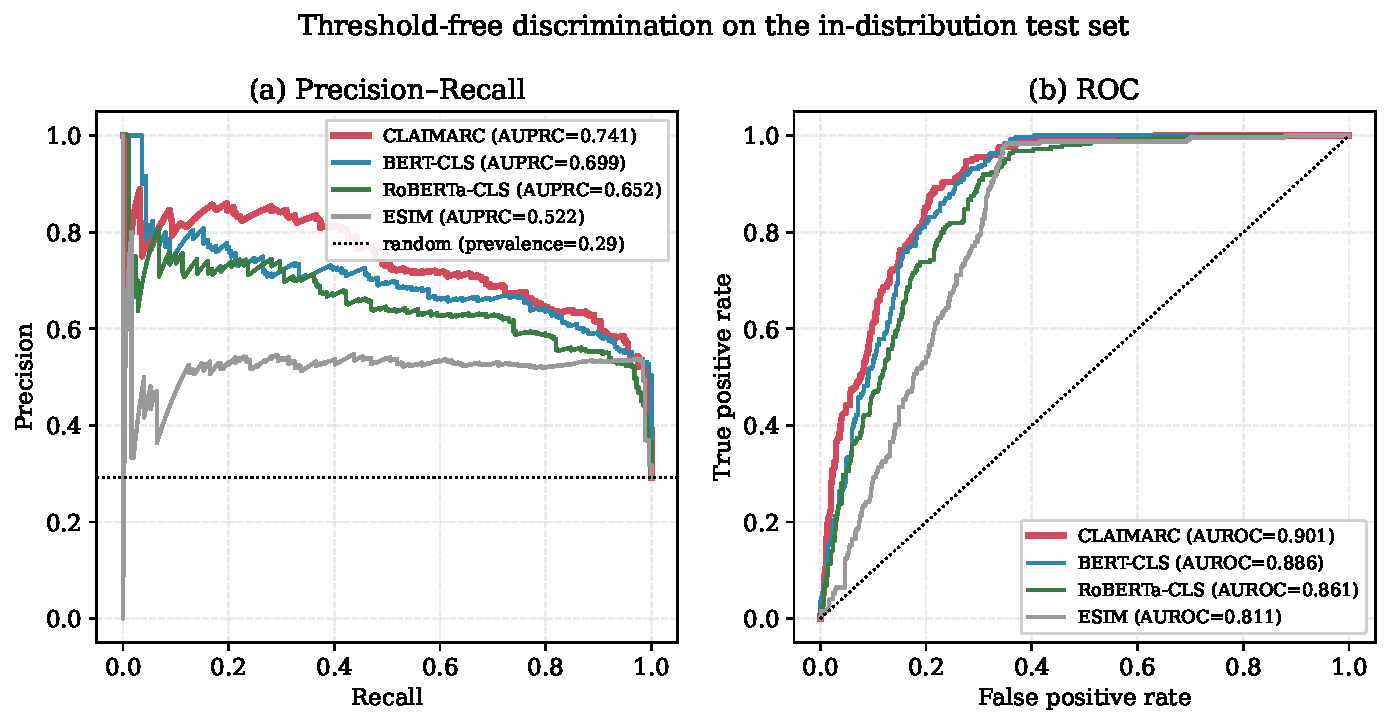
\includegraphics[width=0.86\textwidth]{figs/fig_pr_roc.pdf}
\caption{Threshold-free discrimination on the in-distribution test set.
CLAIMARC (red) dominates the precision--recall curve, particularly in the
high-recall screening regime, and the ROC curve. Dotted line in (a) marks the
positive prevalence ($0.29$).}
\label{fig:prroc}
\end{figure*}

% =====================================================================
\subsection{Ablation Studies (RQ4)}
\label{sec:exp:abl}

Table~\ref{tab:abl} removes one factor at a time from the canonical model,
reported on the two threshold-free primary metrics under a controlled
single-seed protocol. \textbf{Every structural removal lowers both AUPRC and
AUROC}, and the canonical model is strictly best on both, isolating each
component's contribution. The largest drops come from the \textbf{BGE backbone}
($-5.8$ AUPRC vs.\ a BERT backbone), the \textbf{TwoStreamFusion} module
($-4.0$), and \textbf{RACL} ($-4.1$ when the contrastive objective is removed).
Crucially, \textbf{attribute-blocked} hard negatives beat global-pool negatives
($+1.4$ AUPRC), validating the central design that hard negatives must share the
attribute but flip the perceived-risk label. Removing the bidirectional fusion
to a single direction costs $0.4$--$1.2$ AUPRC, and dropping the instance-level
\textbf{reliability weighting} $c_{p,a}$ costs $2.6$ AUPRC---the noisy weak
labels must be discounted. (We note that Macro-F1 is uninformative here: several
ablations match or nominally exceed the full model on Macro-F1 while losing
several AUPRC points, which is precisely why we do not use it,
\S\ref{sec:exp:setup}.)

\begin{table}[t]
\centering\small
\setlength{\tabcolsep}{5pt}
\begin{tabular}{lcccc}
\toprule
\textbf{Ablation} & \textbf{AUPRC} & \textbf{AUROC} & \textbf{$\Delta$AP} & \textbf{$\Delta$AUC} \\
\midrule
\textbf{Canonical CLAIMARC}     & $\mathbf{74.1}$ & $\mathbf{90.1}$ & -- & -- \\
\midrule
\multicolumn{5}{l}{\textit{(1) Backbone \& dual-stream}}\\
\quad backbone: BGE$\to$BERT    & $68.3$ & $88.1$ & $-5.8$ & $-2.0$ \\
\quad w/o TwoStreamFusion       & $70.0$ & $88.6$ & $-4.0$ & $-1.5$ \\
\quad w/o LoRA (full-FT head)   & $71.6$ & $89.8$ & $-2.5$ & $-0.3$ \\
\midrule
\multicolumn{5}{l}{\textit{(2) Fusion mechanism}}\\
\quad x-attn: claim$\to$ev only & $73.7$ & $89.3$ & $-0.4$ & $-0.8$ \\
\quad x-attn: ev$\to$claim only & $72.9$ & $89.1$ & $-1.2$ & $-1.0$ \\
\quad independent projections   & $69.5$ & $88.9$ & $-4.5$ & $-1.2$ \\
\quad FFN: SwiGLU$\to$GELU      & $70.3$ & $87.9$ & $-3.7$ & $-2.2$ \\
\midrule
\multicolumn{5}{l}{\textit{(3) RACL}}\\
\quad w/o contrastive           & $70.0$ & $88.8$ & $-4.1$ & $-1.3$ \\
\quad global-pool hard neg.     & $72.6$ & $89.4$ & $-1.4$ & $-0.6$ \\
\midrule
\multicolumn{5}{l}{\textit{(4) Label \& weighting}}\\
\quad w/o reliability weight $c$ & $71.5$ & $88.4$ & $-2.6$ & $-1.7$ \\
\bottomrule
\end{tabular}
\caption{Component ablations ($\Delta$ vs.\ canonical, single seed). Every
removal degrades both threshold-free metrics; the backbone, dual-stream fusion,
RACL, and attribute-blocked negatives are the largest contributors.}
\label{tab:abl}
\end{table}

% =====================================================================
\subsection{Hyper-parameter Sensitivity and Efficiency (RQ4)}
\label{sec:exp:hyper}

Figure~\ref{fig:hparam} sweeps five core knobs (AUPRC, circle $=$ canonical
setting). The model is \textbf{robust}: AUPRC stays within a narrow
$0.71$--$0.745$ band across all values. The canonical
$\lambda_{\mathrm{CL}}{=}0.5$, $\tau{=}0.07$, $N{=}2$, LoRA rank $16$, and
$(K_p,K_n){=}(3,5)$ sit on the stable plateau; only oversized retrieval sets
$(5,10)$ degrade by importing noisy neighbors.

\paragraph{Efficiency and deployment cost.}
Table~\ref{tab:eff} contrasts CLAIMARC with the strongest encoder and LLM
baselines on deployment-relevant cost. CLAIMARC updates only $92.7$M parameters
($23.4\%$ of its $396.5$M total; the BGE backbone stays frozen) and completes the
full two-stage schedule in $\approx\!13$ min on a single RTX~4090. At inference it
encodes a pair in $36$\,ms and performs attribute-blocked RKC retrieval over the
$3{,}636$-item library in $0.18$\,ms/query (all numbers measured on the same
GPU). Decisively for a constantly-evolving deployment, \emph{adapting to a new
streamer, category, or risk phrasing costs a single $36$\,ms encode plus a
library write---no gradient step}---whereas the parametric baselines require full
or LoRA retraining; the LoRA-SFT Qwen2.5-7B further carries $\sim$$20\times$
CLAIMARC's parameters and autoregressive-decoding latency. This is the
operational payoff of moving the adaptable component from model weights to an
external index.

\begin{table}[t]
\centering\small
\setlength{\tabcolsep}{4pt}
\begin{tabular}{lrrl}
\toprule
\textbf{System} & \textbf{Total} & \textbf{Trainable} & \textbf{New-domain adapt.} \\
\midrule
BERT-base (FT)    & $102$M     & $102$M\,(100\%)             & gradient retrain \\
Qwen2.5-7B+LoRA   & $7{,}616$M & ${\sim}20$M                 & LoRA retrain \\
\textbf{CLAIMARC} & $396.5$M   & $\mathbf{92.7}$M\,(23.4\%)  & \textbf{library write} \\
\bottomrule
\end{tabular}
\caption{Deployment cost. CLAIMARC trains a minority of its parameters and, unlike
the parametric baselines, absorbs new domains by writing to its retrieval library
(one $36$\,ms encode, no gradient update) rather than re-training
(\S\ref{sec:exp:xdom}).}
\label{tab:eff}
\end{table}

\begin{figure}[t]
\centering
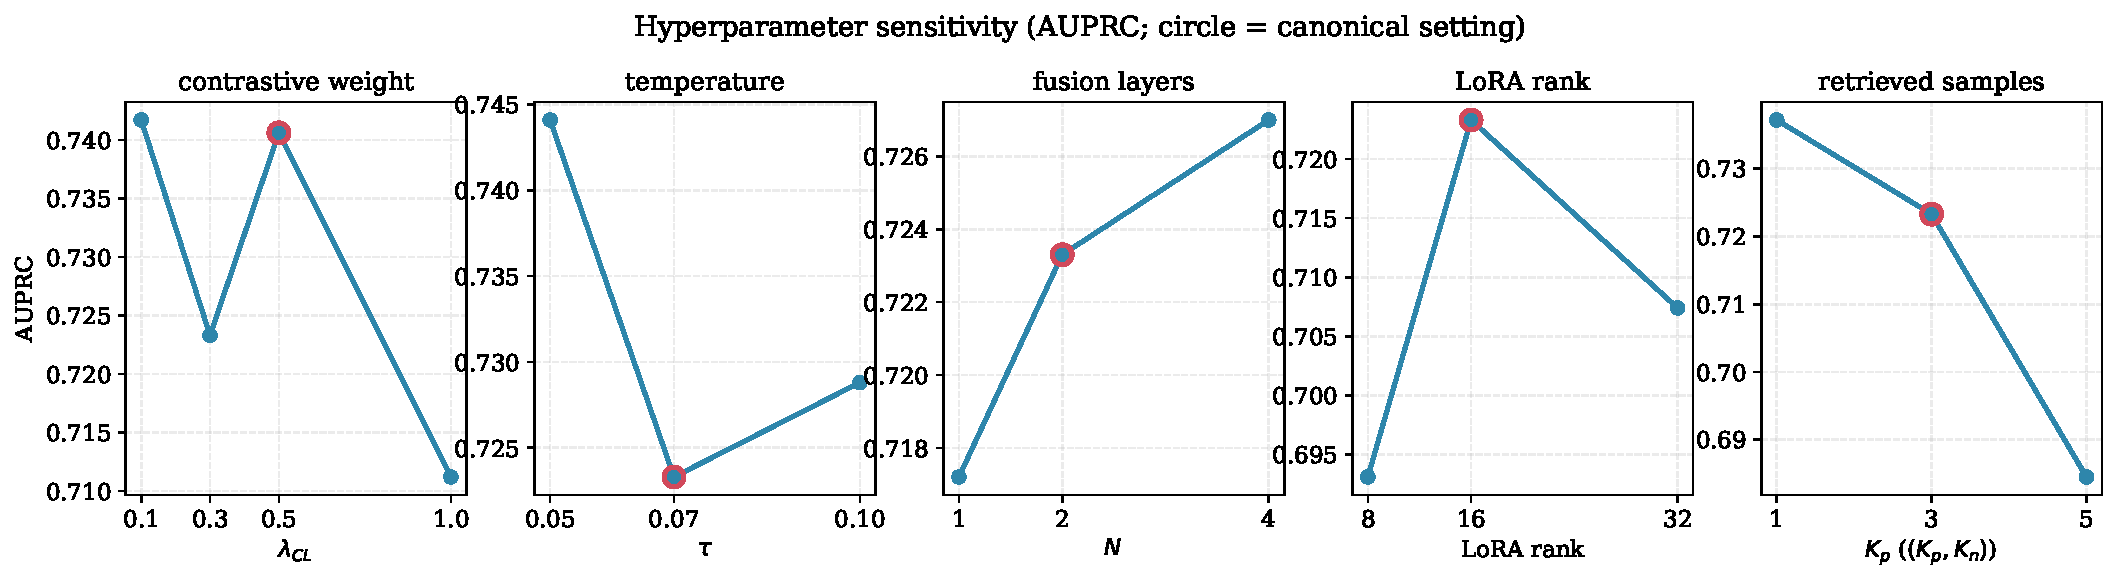
\includegraphics[width=\columnwidth]{figs/fig_hparam.pdf}
\caption{Hyper-parameter sensitivity (AUPRC, single seed). Performance stays
within a narrow band, indicating robustness around the canonical configuration
(circled).}
\label{fig:hparam}
\end{figure}

% =====================================================================
\subsection{Representation Geometry and Boundary Sensitivity (RQ2)}
\label{sec:exp:geom}

To test whether RACL produces the intended geometry, we measure, on the test
retrieval embeddings, the mean cosine to (a) same-attribute \emph{same-label}
neighbors (tightness, higher is better) and (b) same-attribute
\emph{opposite-label} neighbors (separation, \emph{lower} is better)
(Table~\ref{tab:geom}). RACL is decisive: it tightens same-label neighborhoods
($0.62\!\to\!0.72$) and---most importantly---\emph{halves} opposite-label
similarity ($0.275\!\to\!0.133$) relative to the no-contrastive variant, while
attribute-blocked negatives separate opposite labels better than global
negatives ($0.133$ vs.\ $0.152$). The UMAP projection (Fig.~\ref{fig:umap})
visualizes this signature directly: under the full model the perceived-misleading
pairs condense into a clearly detached cluster, whereas without RACL the two
classes are thoroughly interleaved. This is the geometry the framework was
designed to induce---pairs that look alike on objective facts but differ in
consumer perception are pushed apart.

\begin{table}[t]
\centering\small
\setlength{\tabcolsep}{6pt}
\begin{tabular}{lcc}
\toprule
\textbf{Variant} & \textbf{Same-lbl tight}$\uparrow$ & \textbf{Opp-lbl sep}$\downarrow$ \\
\midrule
CLAIMARC w/o RACL        & $0.615$ & $0.275$ \\
CLAIMARC global-neg      & $0.704$ & $0.152$ \\
\textbf{CLAIMARC (full)} & $\mathbf{0.716}$ & $\mathbf{0.133}$ \\
\bottomrule
\end{tabular}
\caption{Attribute-conditioned geometry (test). RACL with attribute-blocked
negatives yields the tightest same-label and best-separated opposite-label
neighborhoods, the mechanism behind the AUPRC gain.}
\label{tab:geom}
\end{table}

\begin{figure}[t]
\centering
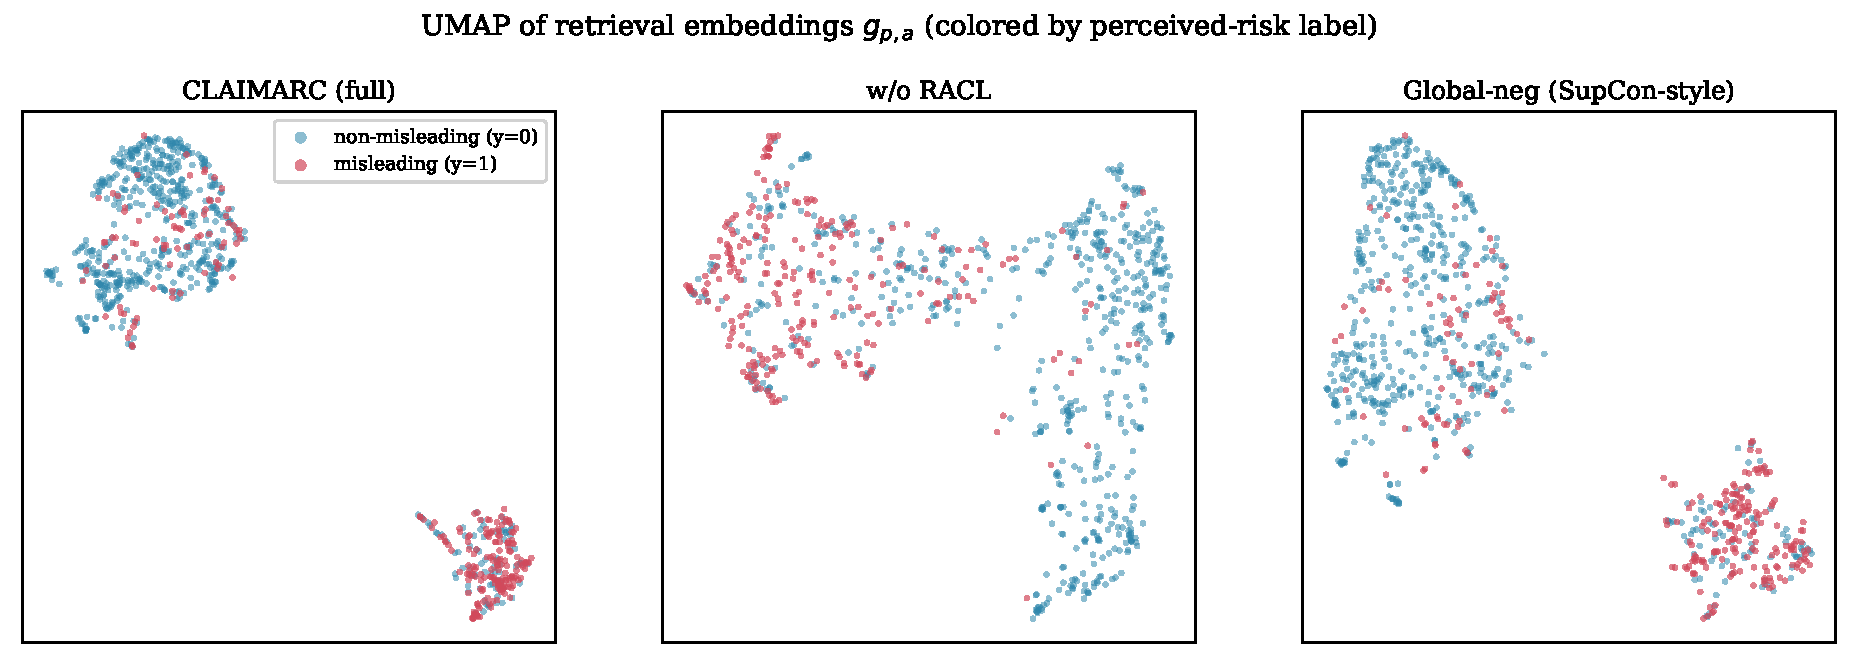
\includegraphics[width=\columnwidth]{figs/fig_umap_label.pdf}
\caption{UMAP of the retrieval embedding $g_{p,a}$ (test), colored by
perceived-risk label. The full model (left) isolates misleading pairs into a
detached cluster; removing RACL (middle) collapses the separation.}
\label{fig:umap}
\end{figure}

\begin{figure}[t]
\centering
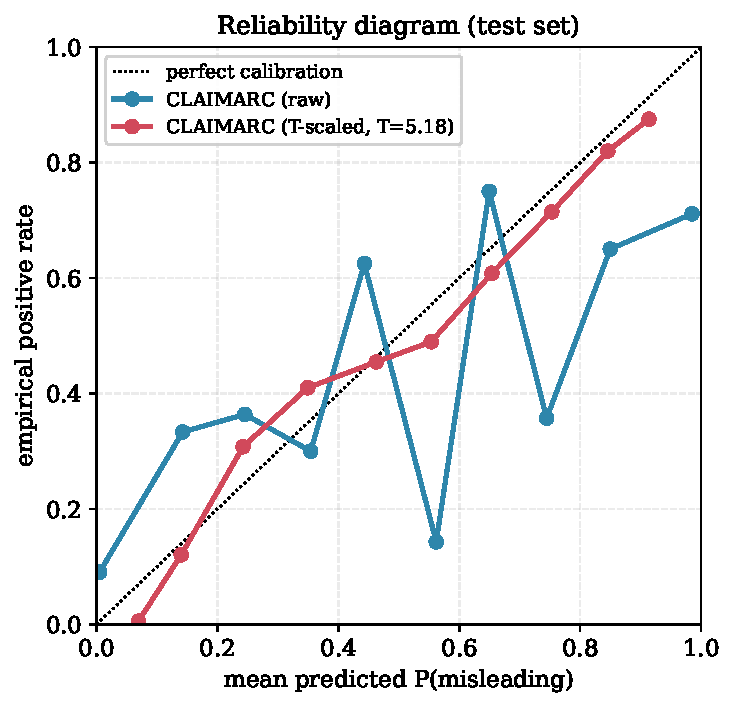
\includegraphics[width=0.82\columnwidth]{figs/fig_calibration.pdf}
\caption{Reliability diagram (test). A single temperature scale brings
CLAIMARC's predicted probabilities close to the diagonal (well calibrated),
supporting their use in a decision-support setting.}
\label{fig:calib}
\end{figure}

% =====================================================================
\subsection{Cross-Domain Generalization (RQ3)}
\label{sec:exp:xdom}

We freeze the encoder/retrieval head after training and evaluate three transfer
protocols (Table~\ref{tab:xdom}), reporting AUPRC. \textbf{Leave-one-category}:
holding out each of the 10 first-level categories in turn, CLAIMARC averages
$70.6$ AUPRC on the unseen category---within $\sim$3 points of the in-domain
$74.1$---with several categories (sports $82.4$, smart-home $77.3$, food $75.1$)
matching or exceeding it, despite never seeing that category in training.
\textbf{Leave-20-streamers}: holding out 20 comment-volume-stratified rooms, it
reaches $77.9$ AUPRC, \emph{above} the in-domain reference, showing no
streamer-identity overfitting and confirming that attribute structure transfers
across streamers even when style does not. \textbf{Time-incremental}: training
only on pre-2025-01 data and testing on the latest period, AUPRC stays high at
$75.0$. Together these confirm the deployment thesis: a frozen encoder plus a
maintained retrieval library generalizes to unseen categories, streamers, and
time without parameter re-training.

\begin{table}[t]
\centering\small
\setlength{\tabcolsep}{6pt}
\begin{tabular}{lc}
\toprule
\textbf{Protocol (frozen encoder)} & \textbf{AUPRC} \\
\midrule
In-domain (reference) & $74.1$ \\
\midrule
Leave-one-category (avg.\ of 10) & $70.6$ \\
\quad best category (sports-and-outdoor) & $82.4$ \\
\quad weakest category (baby-kids-and-pets) & $57.4$ \\
Leave-20-streamers & $77.9$ \\
Time-incremental (test on latest period) & $75.0$ \\
\bottomrule
\end{tabular}
\caption{Cross-domain generalization with a frozen encoder. AUPRC degrades
little---and improves under streamer hold-out---confirming the
library-update adaptation pathway.}
\label{tab:xdom}
\end{table}

% =====================================================================
\subsection{Selective Prediction for Human-in-the-Loop Screening}
\label{sec:exp:select}

A compliance-screening tool is deployed alongside human reviewers, so its
practical value depends not only on average accuracy but on whether it can
\emph{flag its own unreliable decisions} for escalation. CLAIMARC exposes a
natural, training-free gate for this: the \S\ref{sec:exp:setup} forward
classifier and the RKC retrieval vote are two near-independent views of the same
pair, and their disagreement $|p_{\mathrm{fwd}}-p_{\mathrm{RKC}}|$ (the
self-consistency signal of \S3.2.9) marks cases the model should abstain on and
route to a reviewer. Figure~\ref{fig:selective} traces the risk--coverage
trade-off as we abstain on the most-disagreeing pairs. The auto-decided subset
improves \emph{monotonically and substantially}: lowering coverage from $100\%$
to $80\%$ (escalating the $20\%$ highest-disagreement pairs) raises MCC from
$0.586$ to $0.690$, accuracy from $0.809$ to $0.885$, and AUROC from $0.900$ to
$0.938$; at $70\%$ coverage MCC reaches $0.756$ and accuracy $0.920$. A
\emph{random} abstention of the same size leaves every metric flat
($\text{MCC}{\approx}0.585$), confirming that the disagreement gate isolates
genuinely hard cases rather than trivially shrinking the set. The model thus
doubles as a calibrated triage front-end: it can auto-clear the confident
majority and surface a small, high-yield queue for human compliance review.

\begin{figure}[t]
\centering
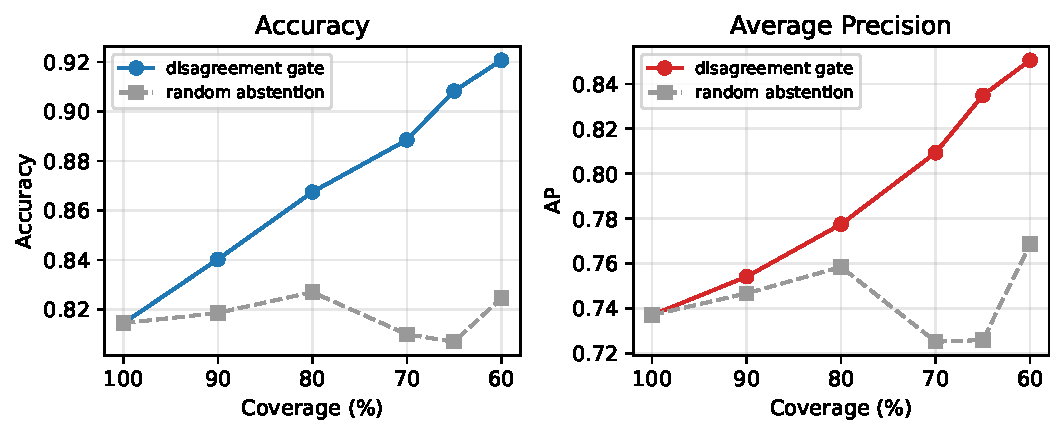
\includegraphics[width=\columnwidth]{figs/fig_selective.pdf}
\caption{Selective prediction on the test set. Abstaining on the highest
forward--RKC disagreement (\S3.2.9) and routing those pairs to human review
sharply improves both (a)~selective AUPRC and (b)~selective MCC on the
auto-decided remainder, whereas random abstention (dashed) is flat. The gate
turns CLAIMARC into a calibrated triage tool.}
\label{fig:selective}
\end{figure}

% =====================================================================
\subsection{Error Analysis}
\label{sec:exp:err}

At the validation-selected operating point CLAIMARC reaches $84\%$ recall on
perceived-misleading pairs (TP$=$210, FN$=$39), trading precision (FP$=$120) as
appropriate for a screening tool. \textbf{Errors concentrate where product
evidence is sparse}: the error rate falls monotonically with evidence-source
coverage ($24.1\%\!\to\!16.4\%\!\to\!10.3\%$ for 1/2/3 sources), underscoring the
value of the three-source product-fact channel and pointing to evidence
acquisition---not the discriminator---as the limiting factor in the residual
regime. The errors fall into two interpretable types. \emph{(i) False
negatives} are dominated by terse \emph{stylized endorsements}
(``\textit{加绒的}'', ``\textit{质感真的很顶}'', ``\textit{版型好看}'')---claims
consumers later judged misleading but that carry no surface contradiction with
the product facts; these are exactly the cases objective fact-verification and
LLM baselines also miss, and the limiting factor is signal sparsity rather than
geometry. \emph{(ii) False positives} concentrate on \emph{hyperbolic metaphor}
over a benign fact (``\textit{喷上去之后就跟镀了膜似的}'' for a foam-type
product), where the model over-attributes risk to vivid figurative language.
Finally, CLAIMARC and BERT make \emph{different} mistakes (each corrects
$\sim$44 of the other's errors, only $114$ jointly wrong), indicating
complementary inductive biases and motivating a retrieval-augmented ensemble as a
natural extension.
